% Created 2021-04-20 Tue 19:43
% Intended LaTeX compiler: pdflatex

\documentclass[english]{article}
\usepackage[T1, T2A]{fontenc}
\usepackage[lutf8]{luainputenc}
\usepackage[english, russian]{babel}
\usepackage{minted}
\usepackage{graphicx}
\usepackage{longtable}
\usepackage{hyperref}
\usepackage{xcolor}
\usepackage{natbib}
\usepackage{amssymb}
\usepackage{stmaryrd}
\usepackage{amsmath}
\usepackage{caption}
\usepackage{mathtools}
\usepackage{amsthm}
\usepackage{tikz}
\usepackage{grffile}
\usepackage{extarrows}
\usepackage{wrapfig}
\usepackage{algorithm}
\usepackage{algorithmic}
\usepackage{lipsum}
\usepackage{rotating}
\usepackage{placeins}
\usepackage[normalem]{ulem}
\usepackage{amsmath}
\usepackage{textcomp}
\usepackage{capt-of}


\usepackage{geometry}
\geometry{a4paper,left=2.5cm,top=2cm,right=2.5cm,bottom=2cm,marginparsep=7pt, marginparwidth=.6in}
 \usepackage{hyperref}
 \hypersetup{
     colorlinks=true,
     linkcolor=blue,
     filecolor=orange,
     citecolor=black,      
     urlcolor=blue,
     }

\date{}
\title{}
\hypersetup{
 pdfauthor={},
 pdftitle={},
 pdfkeywords={},
 pdfsubject={},
 pdfcreator={Emacs 28.0.50 (Org mode 9.4.4)}, 
 pdflang={English}}
\begin{document}

\begin{titlepage}
    \begin{center}
        \large\textbf{Федеральное государственное автономное образовательное учреждение высшего образования ``Национальный исследовательский университет ИТМО``} \\
        \vspace{0.5cm}
        Факультет информационных технологий и программирования \\
        \vspace{0.5cm}
        Направление ``Прикладная математика и информатика`` \\
        \vspace{3cm}
        Отчет к лабораторной работе №2 \\
        \vspace{0.5cm}
        \textbf{Методы многомерной оптимизации}
    \end{center}
    \vfill
    \begin{flushright}
        \large
        Выполнили студенты группы М3237 \\
        \vspace{0.5cm}
        Ярошевский Илья \\
        Аникина Вероника \\
    Крюков Александр
    \end{flushright}
    \vspace{3cm}
    \begin{center}
        Санкт-Петербург 2021
    \end{center}
\end{titlepage}

\section{Цели работы}

\begin{enumerate}
    \item Реализовать алгоритмы
    \begin{itemize}
        \item Метод градиентного спуска
        \item Метод наискорейшего спуска
        \item Метод сопряженных градиентов
    \end{itemize}
    \item Проанализировать траектории методов для некоторых квадратичных функций
    \item Исследовать количество итераций в зависимости от размерности пространства и числа обусловленности
\end{enumerate}
\section{Ход работы}

Во всех тестах начальное приближение --- вектор размерности
пространства из единиц, точность \(\varepsilon\) = 0.001, ограничение на
количество итераций --- 10000 \\
Исходный код: \href{https://github.com/iliayar/MethOpt}{https://github.com/iliayar/MethOpt}
\subsection{Количество итераций}
На графиках:
\begin{itemize}
    \item Горизонтиаль --- число обусловленности
    \item Вертикаль --- количество итераций
\end{itemize}
Для исследования количества итераций использовались случайно
сгенерированные функции вида \(f(x) = \frac{1}{2} A x^2 + b x + c\) с
парамаметрами:
\begin{itemize}
    \item \(A\) --- диагональная матрица с заданным числом обусловленности.
    \item \(b\) --- вектор размерности пространства из единиц.
    \item \(c = 0\)
\end{itemize}
Для каждого числа обусловленности производились тесты на двух
функциях. На графиках представленны средние значения количества
итераций из этих двух тестов.
\subsubsection{Метод градиентного спуска}
\begin{center}
    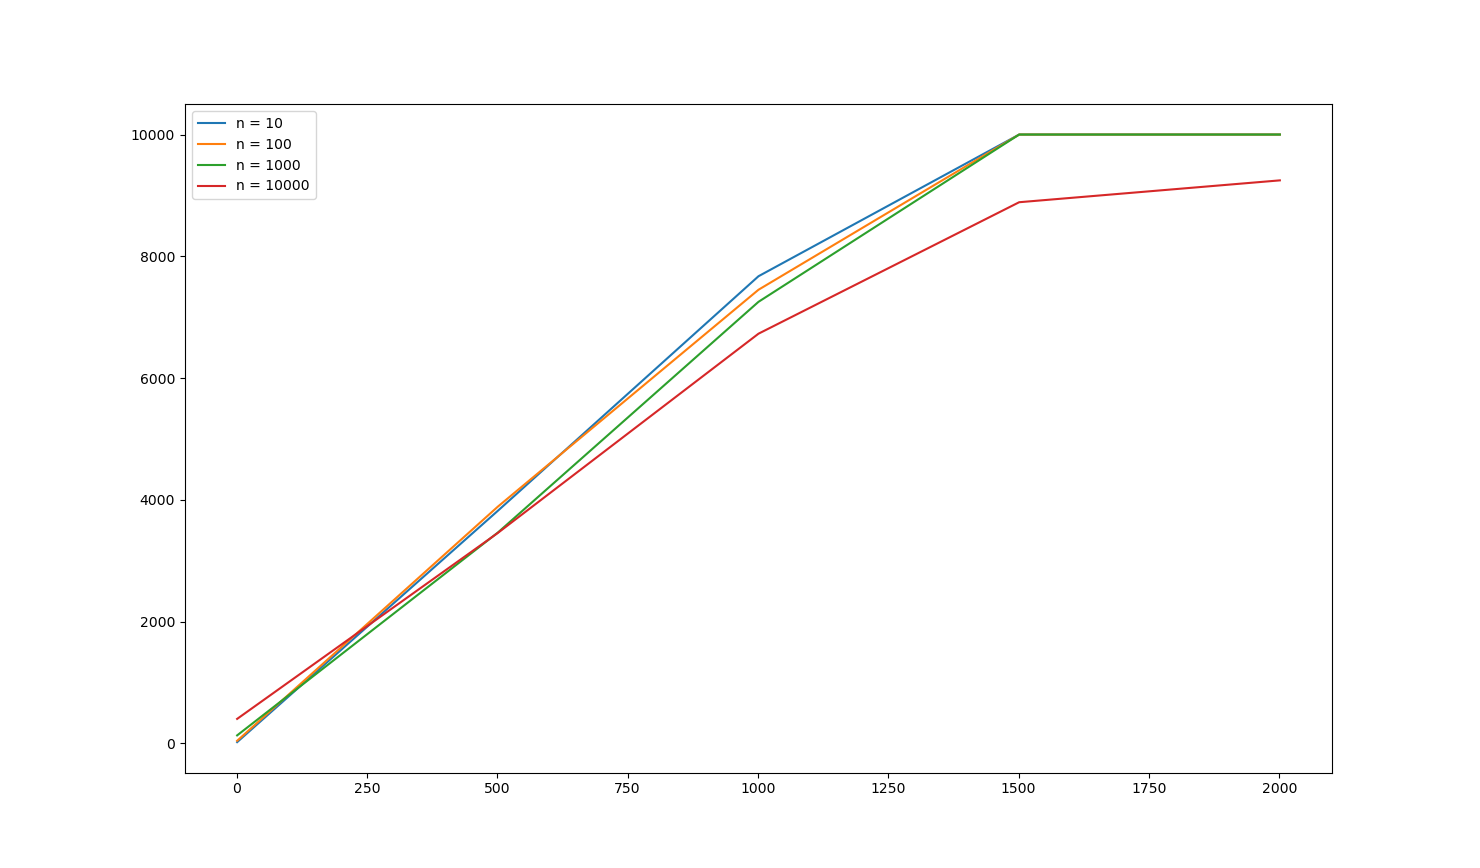
\includegraphics[scale=0.4]{plots/gradient_descent_1.png}
\end{center} 
Видно, что количество итераций не
зависит от размерности пространства \(n\), но линейно зависит от числа
обусловленности \(k\)

\subsubsection{Метод наискорейшего спуска}

\begin{center}
    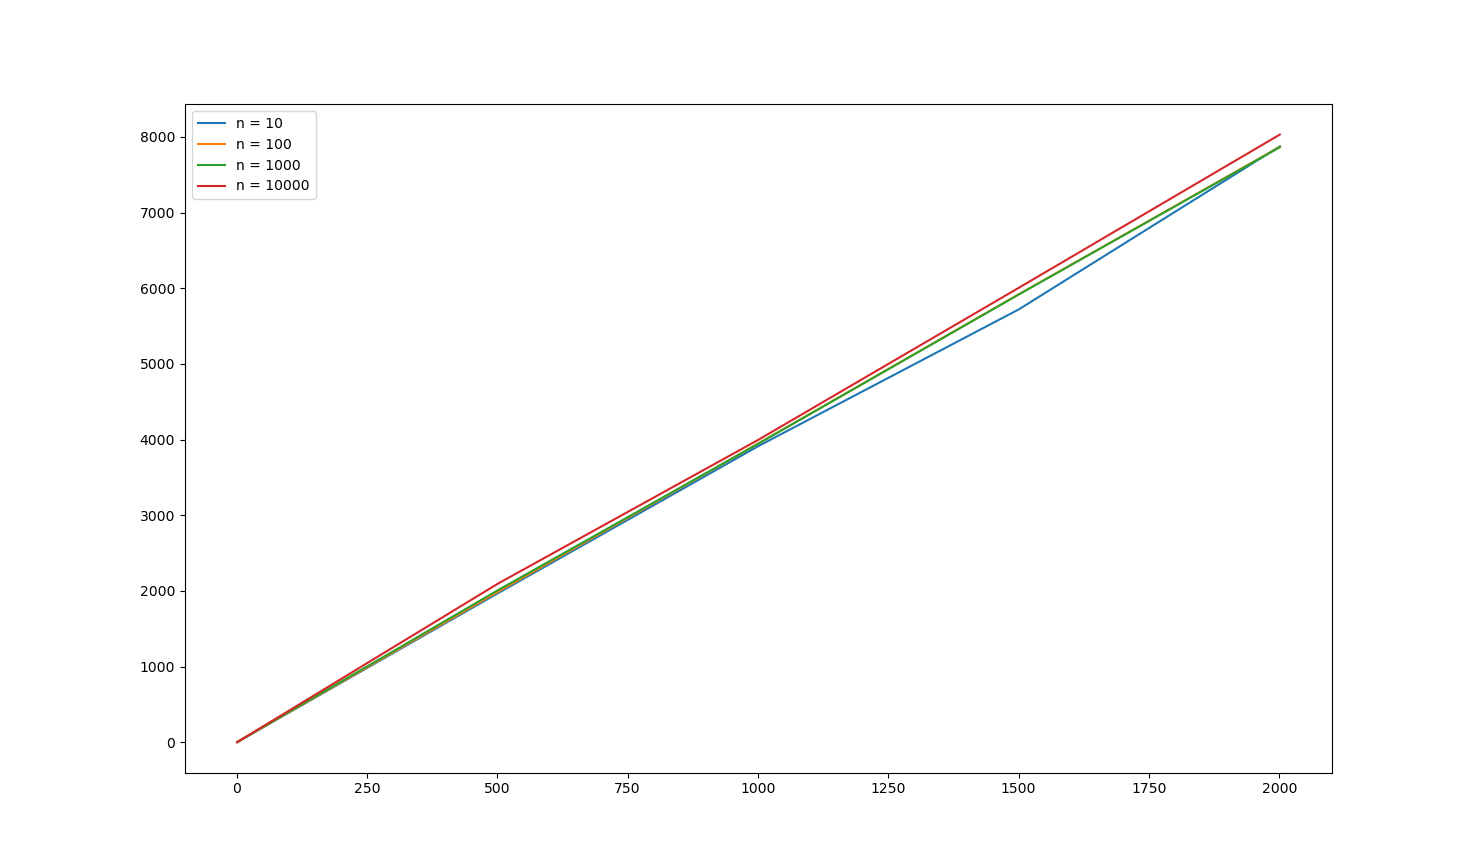
\includegraphics[scale=0.4]{plots/steepest_gradient_1.png}
\end{center} 
Так же как и в методе градиентного
спуска можно видеть линейную зависимость количества итераций от числа
обусловленности. Количество итераций так же не зависит от размерности
пространства.

Исследование зависимости количества итераций методов одномерной
оптимизации от числа обусловленности \(k\) матрицы \(A\) и размерности
пространства \(n\):
\begin{center}
  \begin{longtable}{l|lllll}
    \(k\) & Дихотомии & Парабол & Золотого сечения & Брента & Метод Фибоначчи \\
    \hline
    1 & 62.0 & 12.0 & 46.0 & 28.0 & 50.0 \\
    101 & 62.0 & 12.0 & 46.0 & 45.59620962038987 & 50.0 \\
    201 & 62.0 & 12.0 & 46.0 & 48.28764921658471 & 50.0 \\
    301 & 62.0 & 12.0 & 46.0 & 49.76634216945256 & 50.0 \\
    401 & 62.0 & 12.0 & 46.0 & 50.20143294461716 & 50.0 \\
    501 & 62.0 & 12.0 & 46.0 & 51.98284088537922 & 50.0 \\
    601 & 62.0 & 12.0 & 46.0 & 52.832648532326026 & 50.0 \\
    701 & 62.0 & 12.0 & 46.0 & 52.90359065326178 & 50.0 \\
    801 & 62.0 & 12.0 & 46.0 & 53.742663849573695 & 50.0 \\
    901 & 62.0 & 12.0 & 46.0 & 54.71023523481371 & 50.0 \\
    \caption{Зависимость количества итераций одномерной оптимизации от числа обусловленности}
  \end{longtable}
\end{center}
\begin{center}
  \begin{longtable}{l|lllll}
    \(n\) & Дихотомии & Парабол & Золотого сечения & Брента & Метод Фибоначчи \\
    \hline
    1 & 18.6 & 3.6 & 13.8 & 8.4 & 15.0 \\
    101 & 18.6 & 3.6 & 13.8 & 11.194634715687346 & 15.0 \\
    201 & 18.6 & 3.6 & 13.8 & 11.109615384615385 & 15.0 \\
    301 & 18.6 & 3.6 & 13.8 & 11.166219512195124 & 15.0 \\
    401 & 18.6 & 3.6 & 13.8 & 11.10060975609756 & 15.0 \\
    501 & 18.6 & 3.6 & 13.8 & 11.143670150987225 & 15.0 \\
    601 & 18.6 & 3.6 & 13.8 & 11.078048780487805 & 15.0 \\
    \caption{Зависимость количества итераций одномерной оптимизации от размерности пространства}
  \end{longtable}
\end{center}
Как видно, все методы, кроме метода Брента, не зависит ни от
размерности пространства, ни от числа обусловленности. Метод Брента
почти не зависит от размерности и линейно зависит от числа
обусловленности

Исследование количества итераций метода наискорейшего спуска от выбора
метода одномерной оптимизации, размерности пространства и числа
обусловленности
\begin{center}
  \begin{longtable}{l|lllll}
    \(k\) & Дихотомии & Парабол & Золотого сечения & Брента & Метод Фибоначчи \\
    \hline
    1 & 0.6 & 0.6 & 0.6 & 0.6 & 0.6 \\
    101 & 139.8 & 165.0 & 181.4 & 165.0 & 169.4 \\
    201 & 347.2 & 261.2 & 310.0 & 261.2 & 424.6 \\
    301 & 531.8 & 462.0 & 529.4 & 462.0 & 611.0 \\
    401 & 844.6 & 777.8 & 860.0 & 777.8 & 767.6 \\
    501 & 1018.0 & 918.4 & 938.8 & 918.4 & 1009.4 \\
    601 & 1208.4 & 1011.4 & 1093.2 & 1011.4 & 1290.4 \\
    701 & 1495.2 & 1017.2 & 1412.2 & 1017.2 & 1188.8 \\
    801 & 986.2 & 1429.4 & 1452.4 & 1429.4 & 932.6 \\
    901 & 1907.2 & 1687.4 & 1876.6 & 1687.4 & 1282.8 \\
    \caption{Зависимость количества итераций многомерной оптимизации от числа обусловленности для каждого метода одномерной оптимизации}
  \end{longtable}
\end{center}
\begin{center}
  \begin{longtable}{l|lllll}
    \(k\) & Дихотомии & Парабол & Золотого сечения & Брента & Метод Фибоначчи \\
    \hline
    1 & 1.2 & 0.6 & 1.2 & 0.6 & 1.2 \\
    101 & 23.2 & 23.2 & 23.2 & 23.2 & 23.2 \\
    201 & 23.4 & 23.4 & 23.4 & 23.4 & 23.4 \\
    301 & 24.2 & 24.0 & 24.2 & 24.0 & 24.0 \\
    401 & 24.4 & 24.4 & 24.4 & 24.4 & 24.4 \\
    \caption{Зависимость количества итераций многомерной оптимизации от размерности пространства для каждого метода одномерной оптимизации}
  \end{longtable}
\end{center}

Как видно количество итераций в зависимости от размерности
пространства для каждого метода одномерной оптимизации
одинаково. Зависимость же от числа обусловленности для каждого метода
имеет довольно сильный разброс, но в целом нельзя сказать что выбор
какого-то метода одномерной оптимизации ведет к меньшему числу
многомерных итераций

Можно сказать что метод парабол оказывается лучше других почти по всем параметрам

\subsubsection{Метод сопряженный градиентов}
\begin{center}
    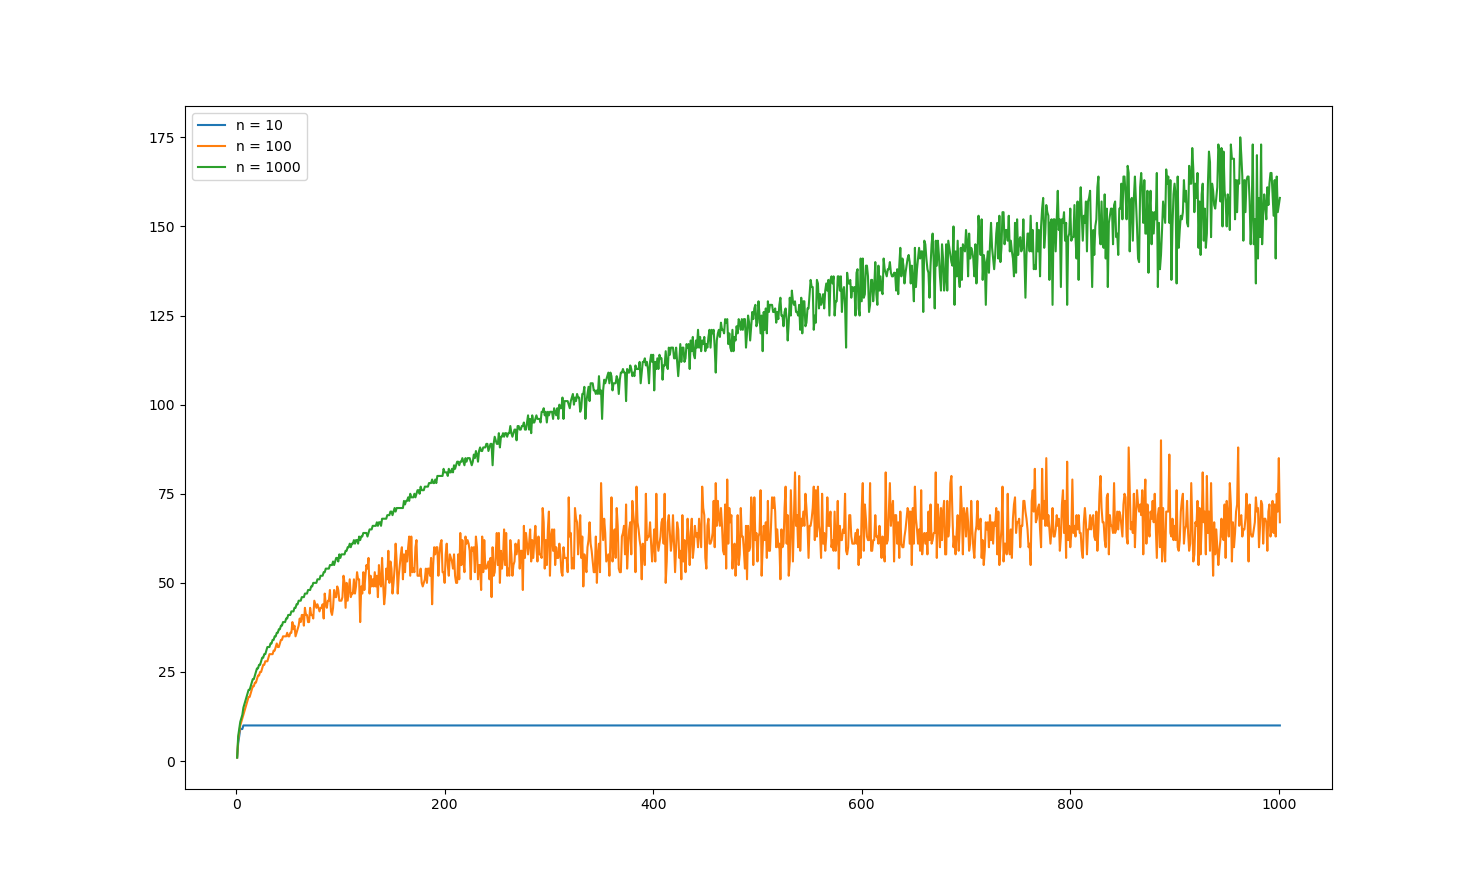
\includegraphics[scale=0.4]{plots/conjugate_gradient_1.png}
\end{center}
Видно что количество итераций нелинейно зависит от числа
обусловленности и довольно сильно зависит от размерности
пространства. Так же можно отметить, что количество итераций всегда
будет не больше размерности пространства.

Посмотрим как выбирается величина шага \(\alpha\) на каждой итерации

\subsection{Траектории}
\[ f_1(x) = \frac{1}{2}\begin{pmatrix}
100 & -1 \\
-1 & 1
\end{pmatrix} x^2 + \begin{pmatrix} -10 & 0 \end{pmatrix}x\]
Все методы находят минимум функции \(f_1^* = -0.50505\) в точке \(x^* = (0.101011\ 0.1011)\)
\[ f_2(x) = \frac{1}{2}\begin{pmatrix}
3 & -1 \\
-1 & 2
\end{pmatrix} x^2 + \begin{pmatrix} -5 & 2 \end{pmatrix}x\]
Все методы находят минимум функции \(f_2^* = -4.2\) в точке \(x^* = (1.6\ -0.2)\)
\[ f_3(x) = \frac{1}{2}\begin{pmatrix}
1 & -1 \\
-1 & 2
\end{pmatrix} x^2 + \begin{pmatrix} -10 & 2 \end{pmatrix}x\]
Все методы находят минимум функции \(f_3^* = -82\) в точке \(x^* = (18\ 8)\) \\

\subsubsection{Метод градиентного спуска}
\begin{center}
    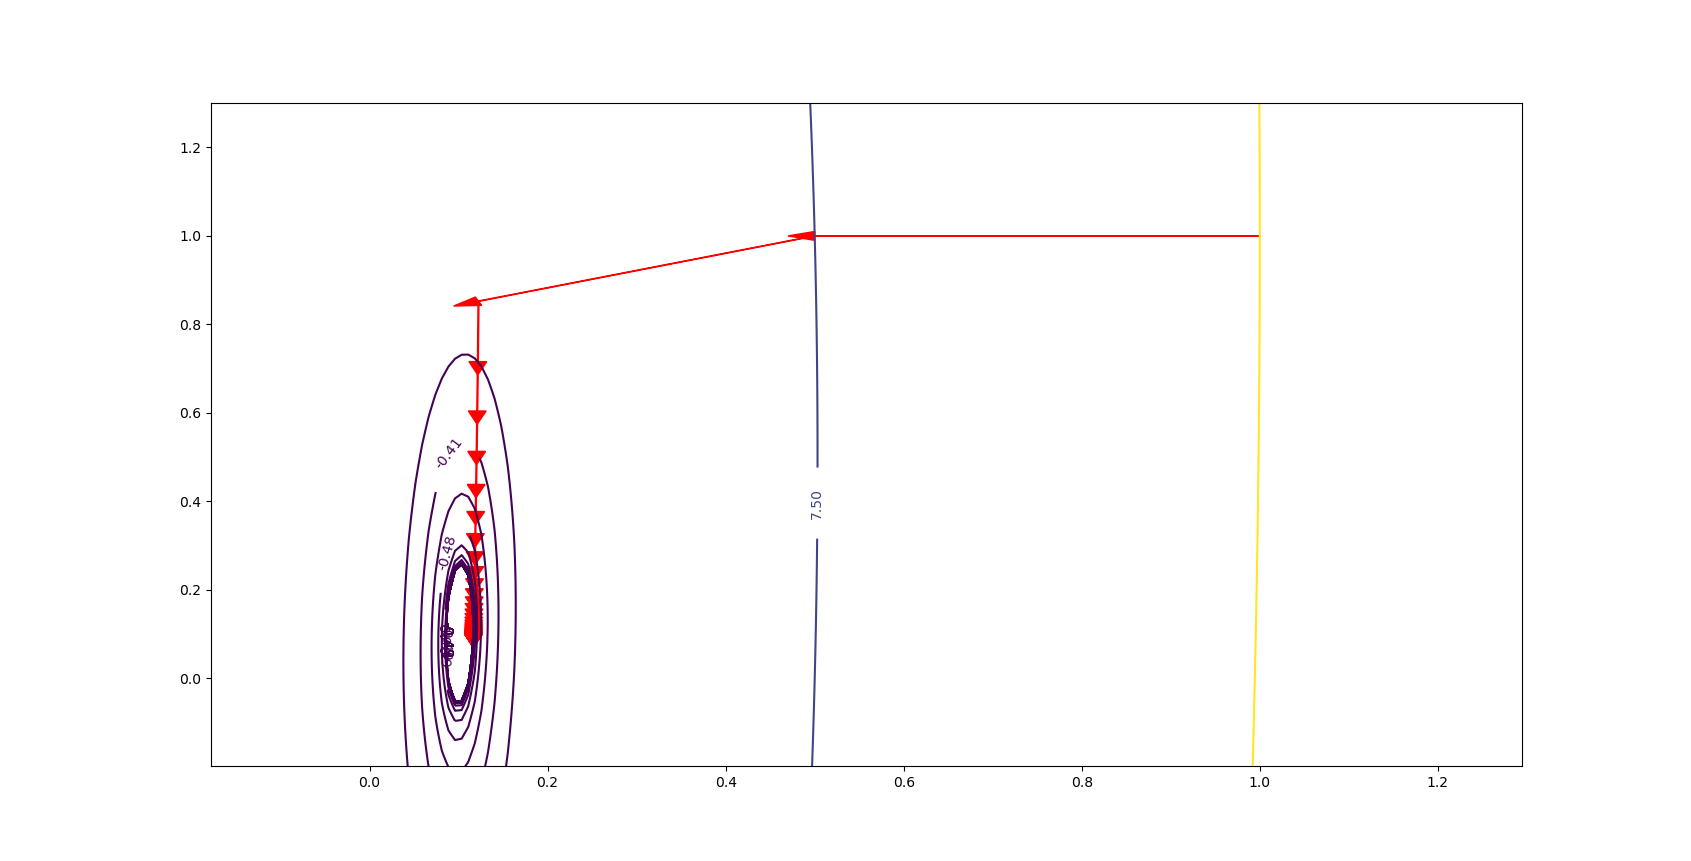
\includegraphics[scale=0.3]{plots/traectories/gradient_descent_1.png}
    \captionof{figure}{Траектория метода на функции \(f_1\)}
\end{center}
\begin{center}
    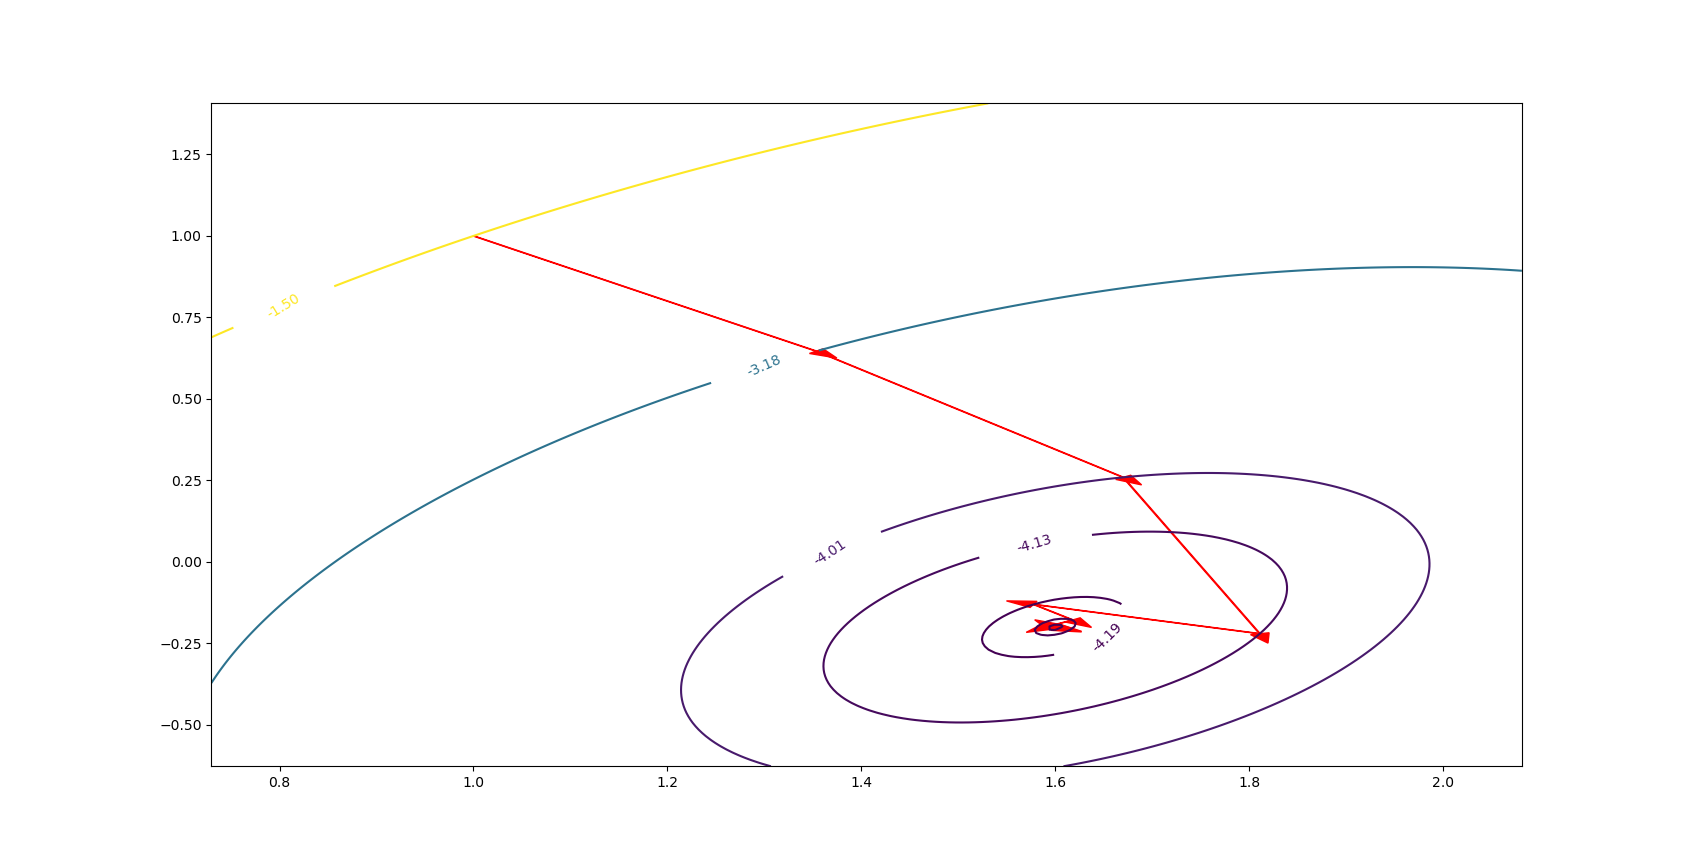
\includegraphics[scale=0.3]{plots/traectories/gradient_descent_2.png}
    \captionof{figure}{Траектория метода на функции \(f_2\)}
\end{center}
\begin{center}
    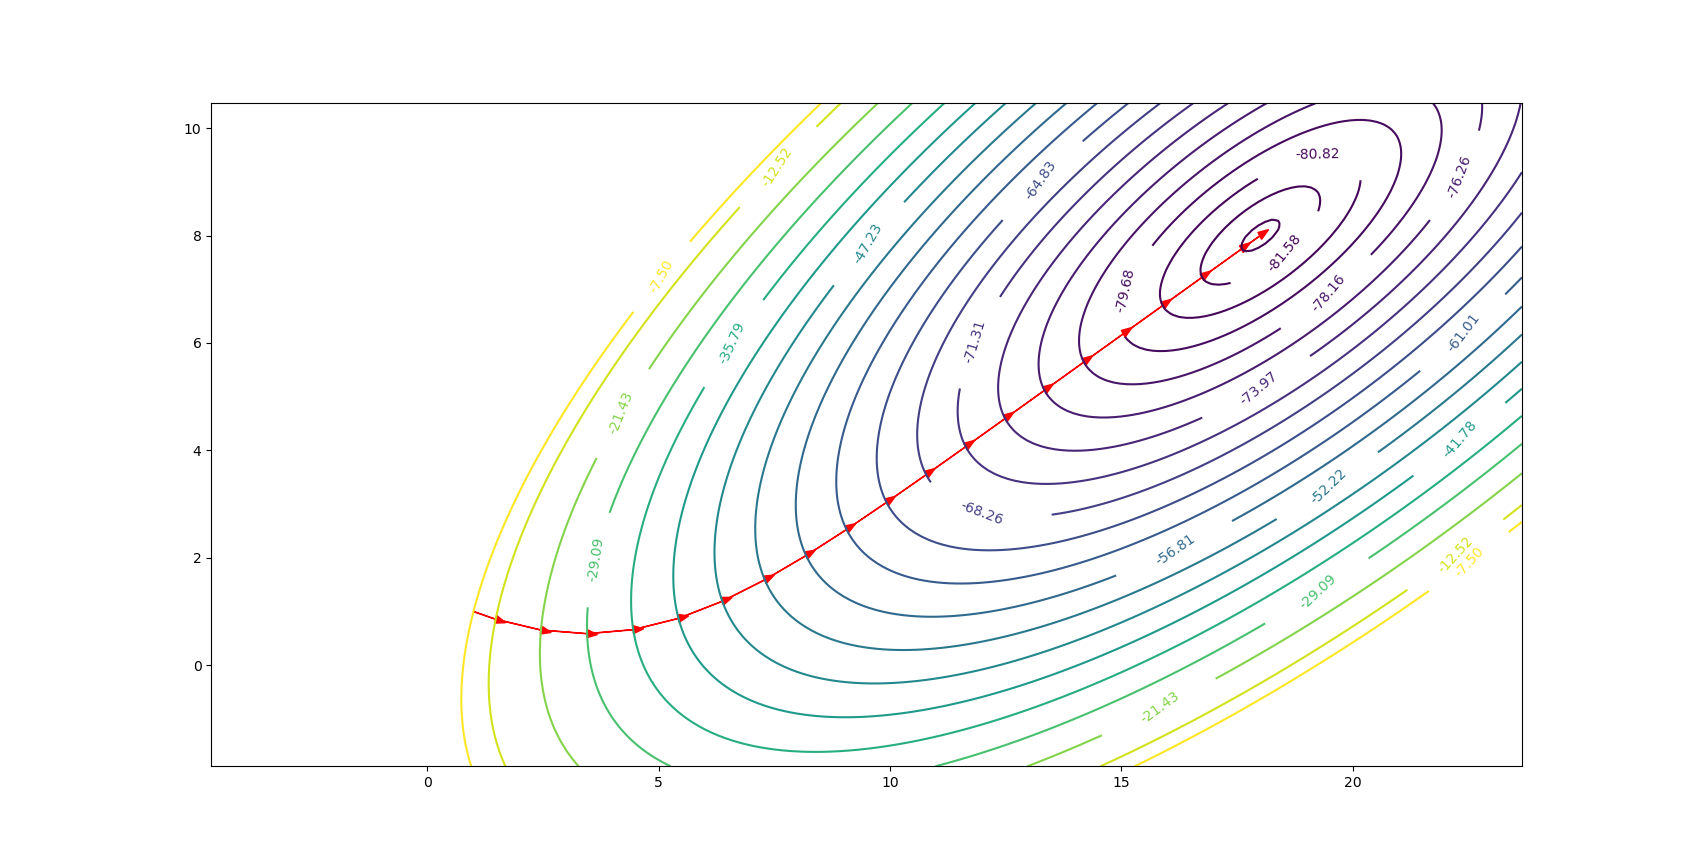
\includegraphics[scale=0.3]{plots/traectories/gradient_descent_3.png}
    \captionof{figure}{Траектория метода на функции \(f_3\)}
\end{center}

При запуске на \(f_1\) методу потребовалось гораздо больше шагов
(\(\approx\) 800) дла нахождения минимума в отличии от функций \(f_2\)
(\(\approx\) 10 шагов) и \(f_1\) (\(\approx\) 40 шагов), так как число
обусловленности матрицы \(A\) функции \(f_1\) достаточно велико \(\mu
= 100\).
\subsubsection{Метод наискорейшего спуска}
\begin{center}
    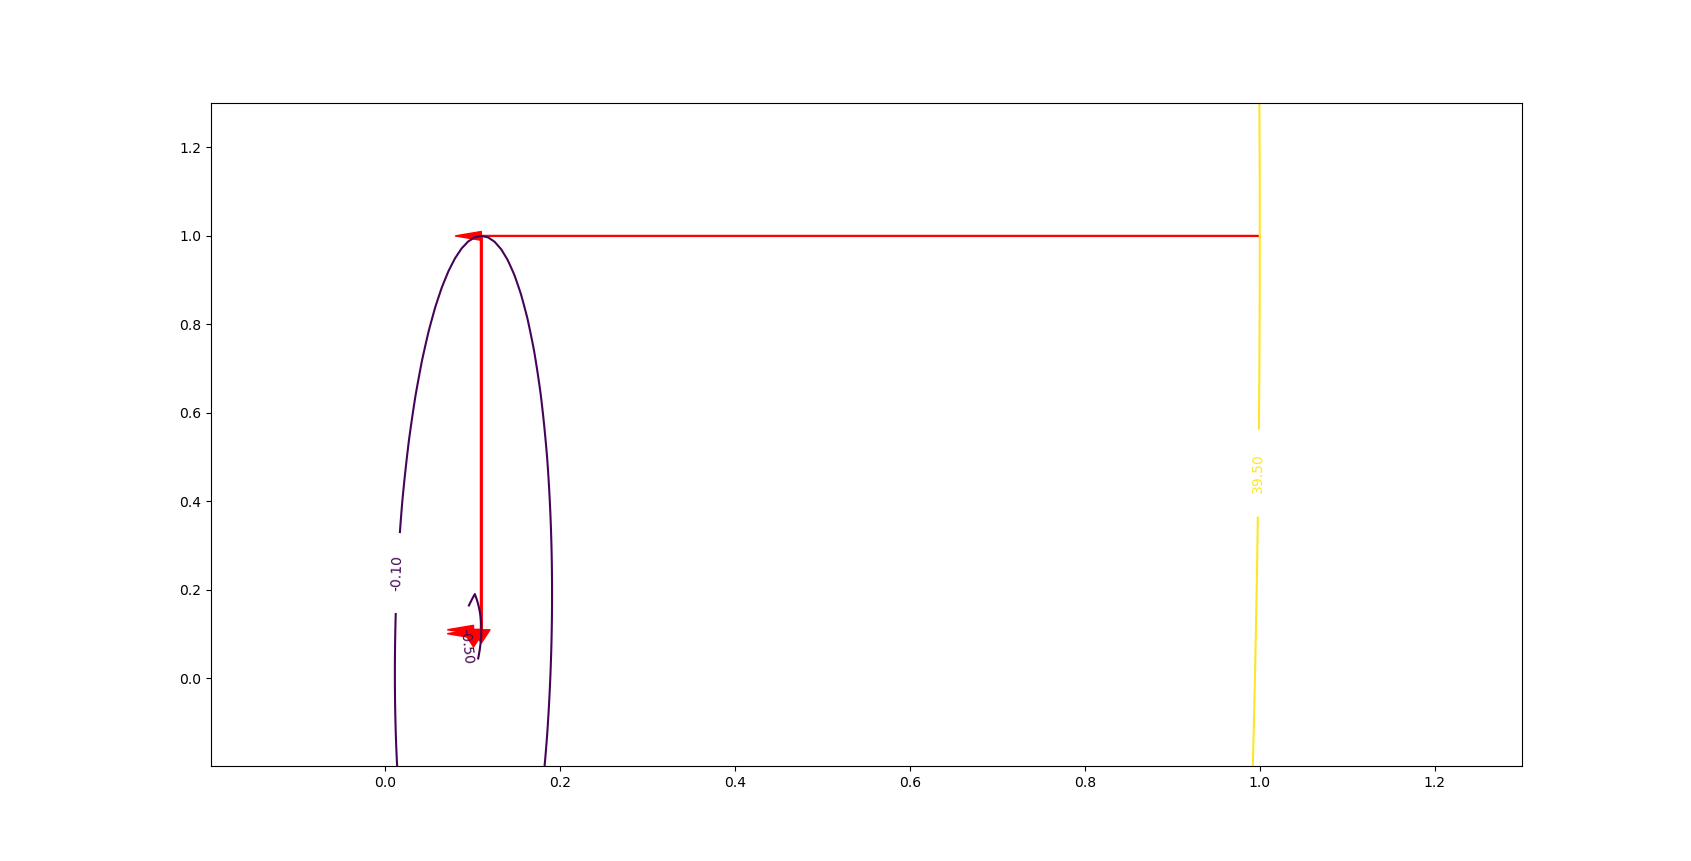
\includegraphics[scale=0.3]{plots/traectories/steepest_descent_1.png}
    \captionof{figure}{Траектория метода на функции \(f_1\)}
\end{center}
\begin{center}
    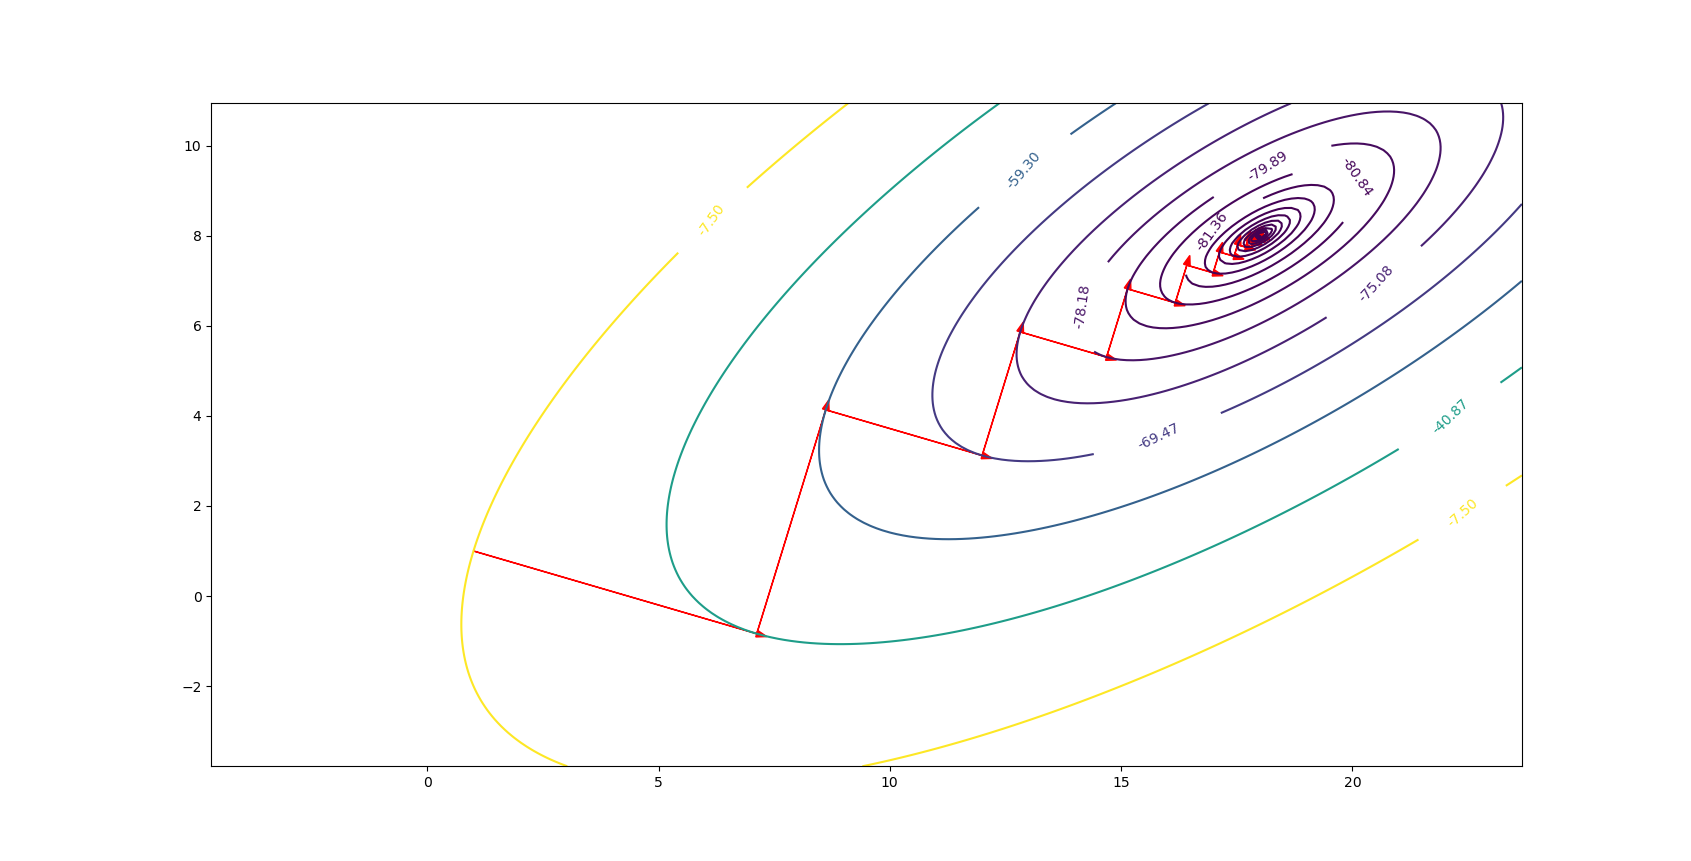
\includegraphics[scale=0.3]{plots/traectories/steepest_descent_3.png}
    \captionof{figure}{Траектория метода на функции \(f_3\)}
\end{center}

Не смотря на высокое число обусловленности функции \(f_1\), метод
потребовалось 5 шагов для нахождения минимума. Но в то же время на
функции \(f_3\) потребовалось всего 2 шага.

\subsubsection{Метод сопряженных градиентов}
\begin{center}
    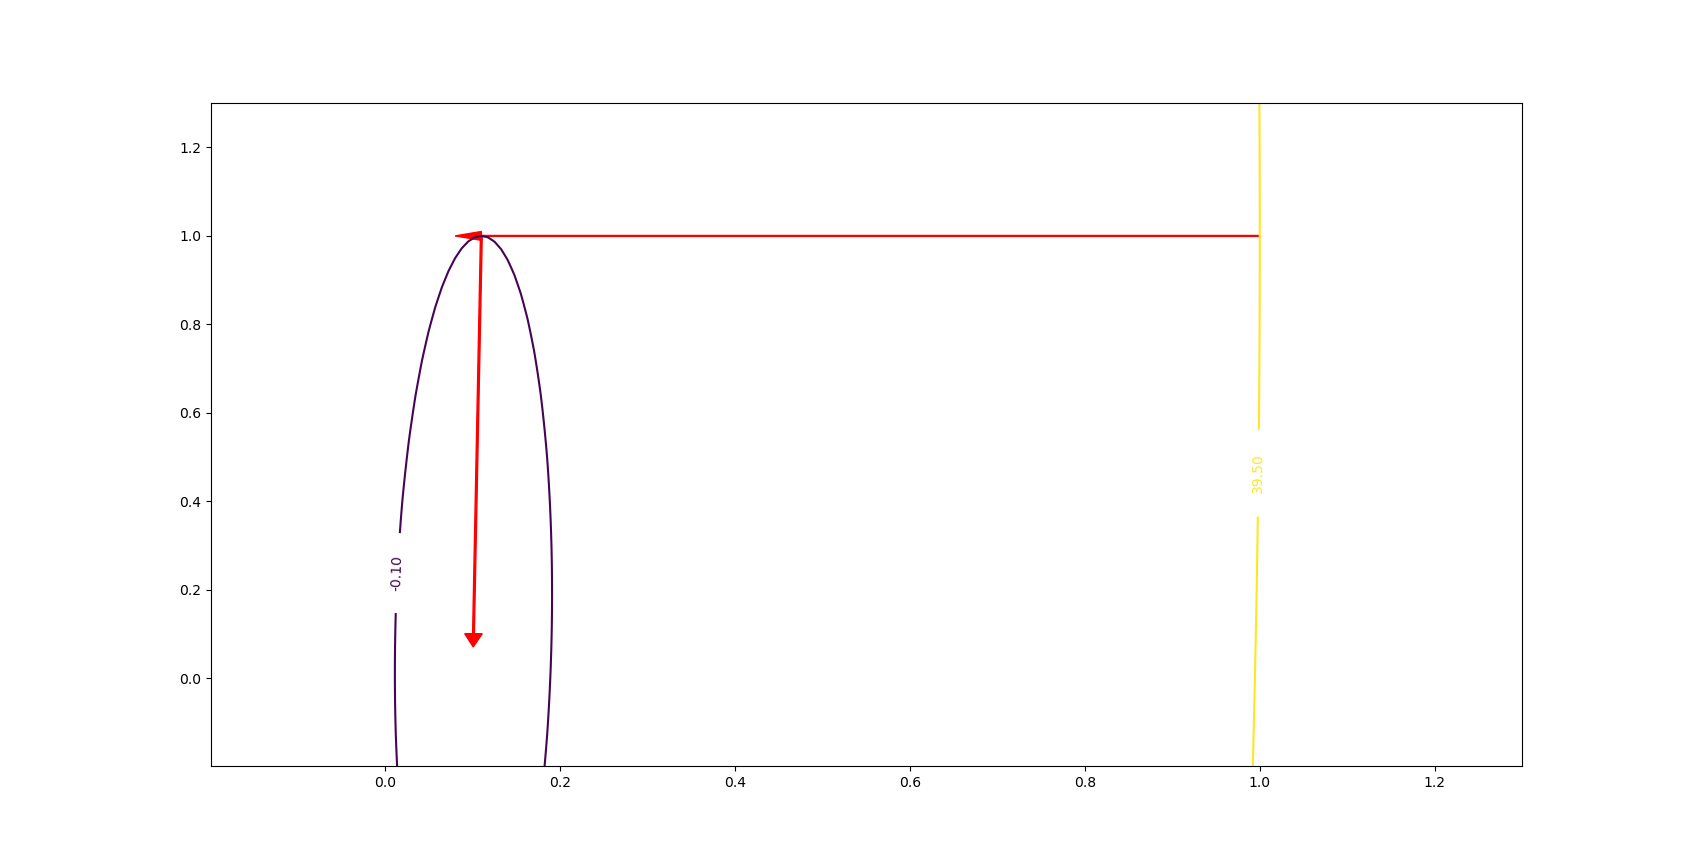
\includegraphics[scale=0.3]{plots/traectories/conjugate_gradient_1.png}
    \captionof{figure}{Траектория метода на функции \(f_1\)}
\end{center}
\begin{center}
    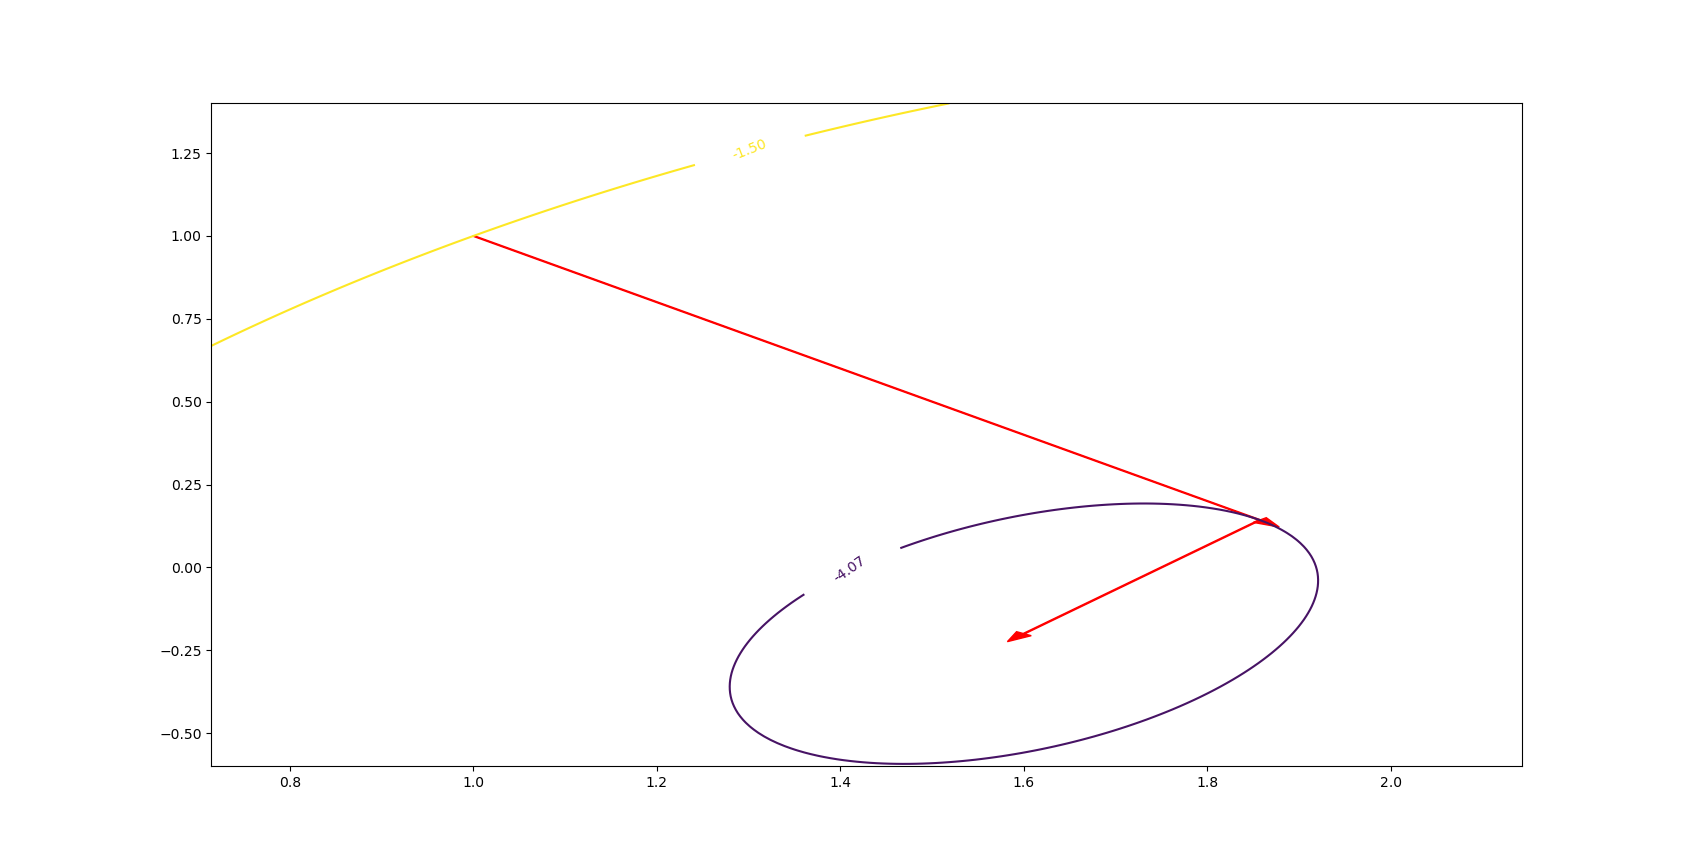
\includegraphics[scale=0.3]{plots/traectories/conjugate_gradient_2.png}
    \captionof{figure}{Траектория метода на функции \(f_2\)}
\end{center}
\[ f_0(x) = \frac{1}{2}\begin{pmatrix}2 & -1 \\ -1 & 2\end{pmatrix}x^2 \quad x^0 = (1, 1) \]
\begin{center}
    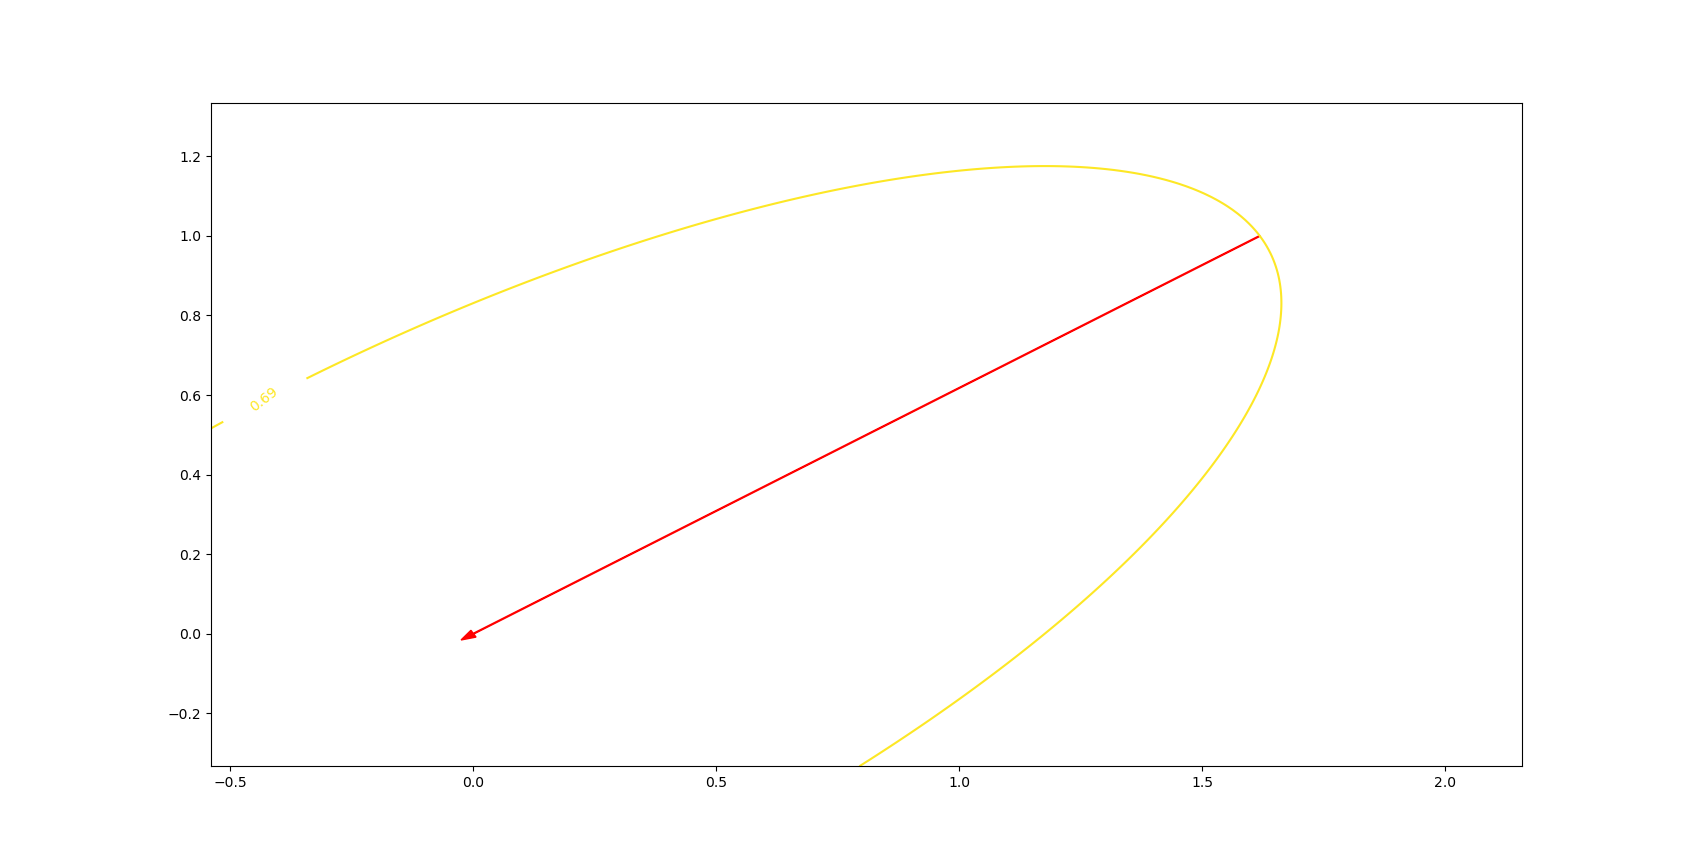
\includegraphics[scale=0.3]{plots/traectories/conjugate_gradient_3.png}
    \captionof{figure}{Траектория метода на функции \(f_0\) с начальным приближением \(x_0\)}
\end{center}

Данный метод находит точку минимума на заданных функциях за два или
три шага. В случае 3, когда начальное приближение равно собственному
вектору матрицы \(A\) и \(b = (0, 0)\), метод находит точку минимума
за один шаг. Это свойство также будет верно и для метода сопряженных
градиентов.

\section{Выводы}
Больше всего итераций совершает метод градиентоного спуска. Он линейно
зависит от числа обусловленности, но коэффицент этой зависимости
больше чем у метода наискорейшего спуска. Лучше всего себя показывает
метод сопряженных градиентов. Он совершает меньше всего итераций до
сходимости, а также имеет не линейную зависимость от числа
обусловленности. Но главная особенность --- он имеет верхную границу
числа итераций равную размрности пространства.

\end{document}
